% Created by tikzDevice version 0.12.3.1 on 2021-11-28 16:40:08
% !TEX encoding = UTF-8 Unicode
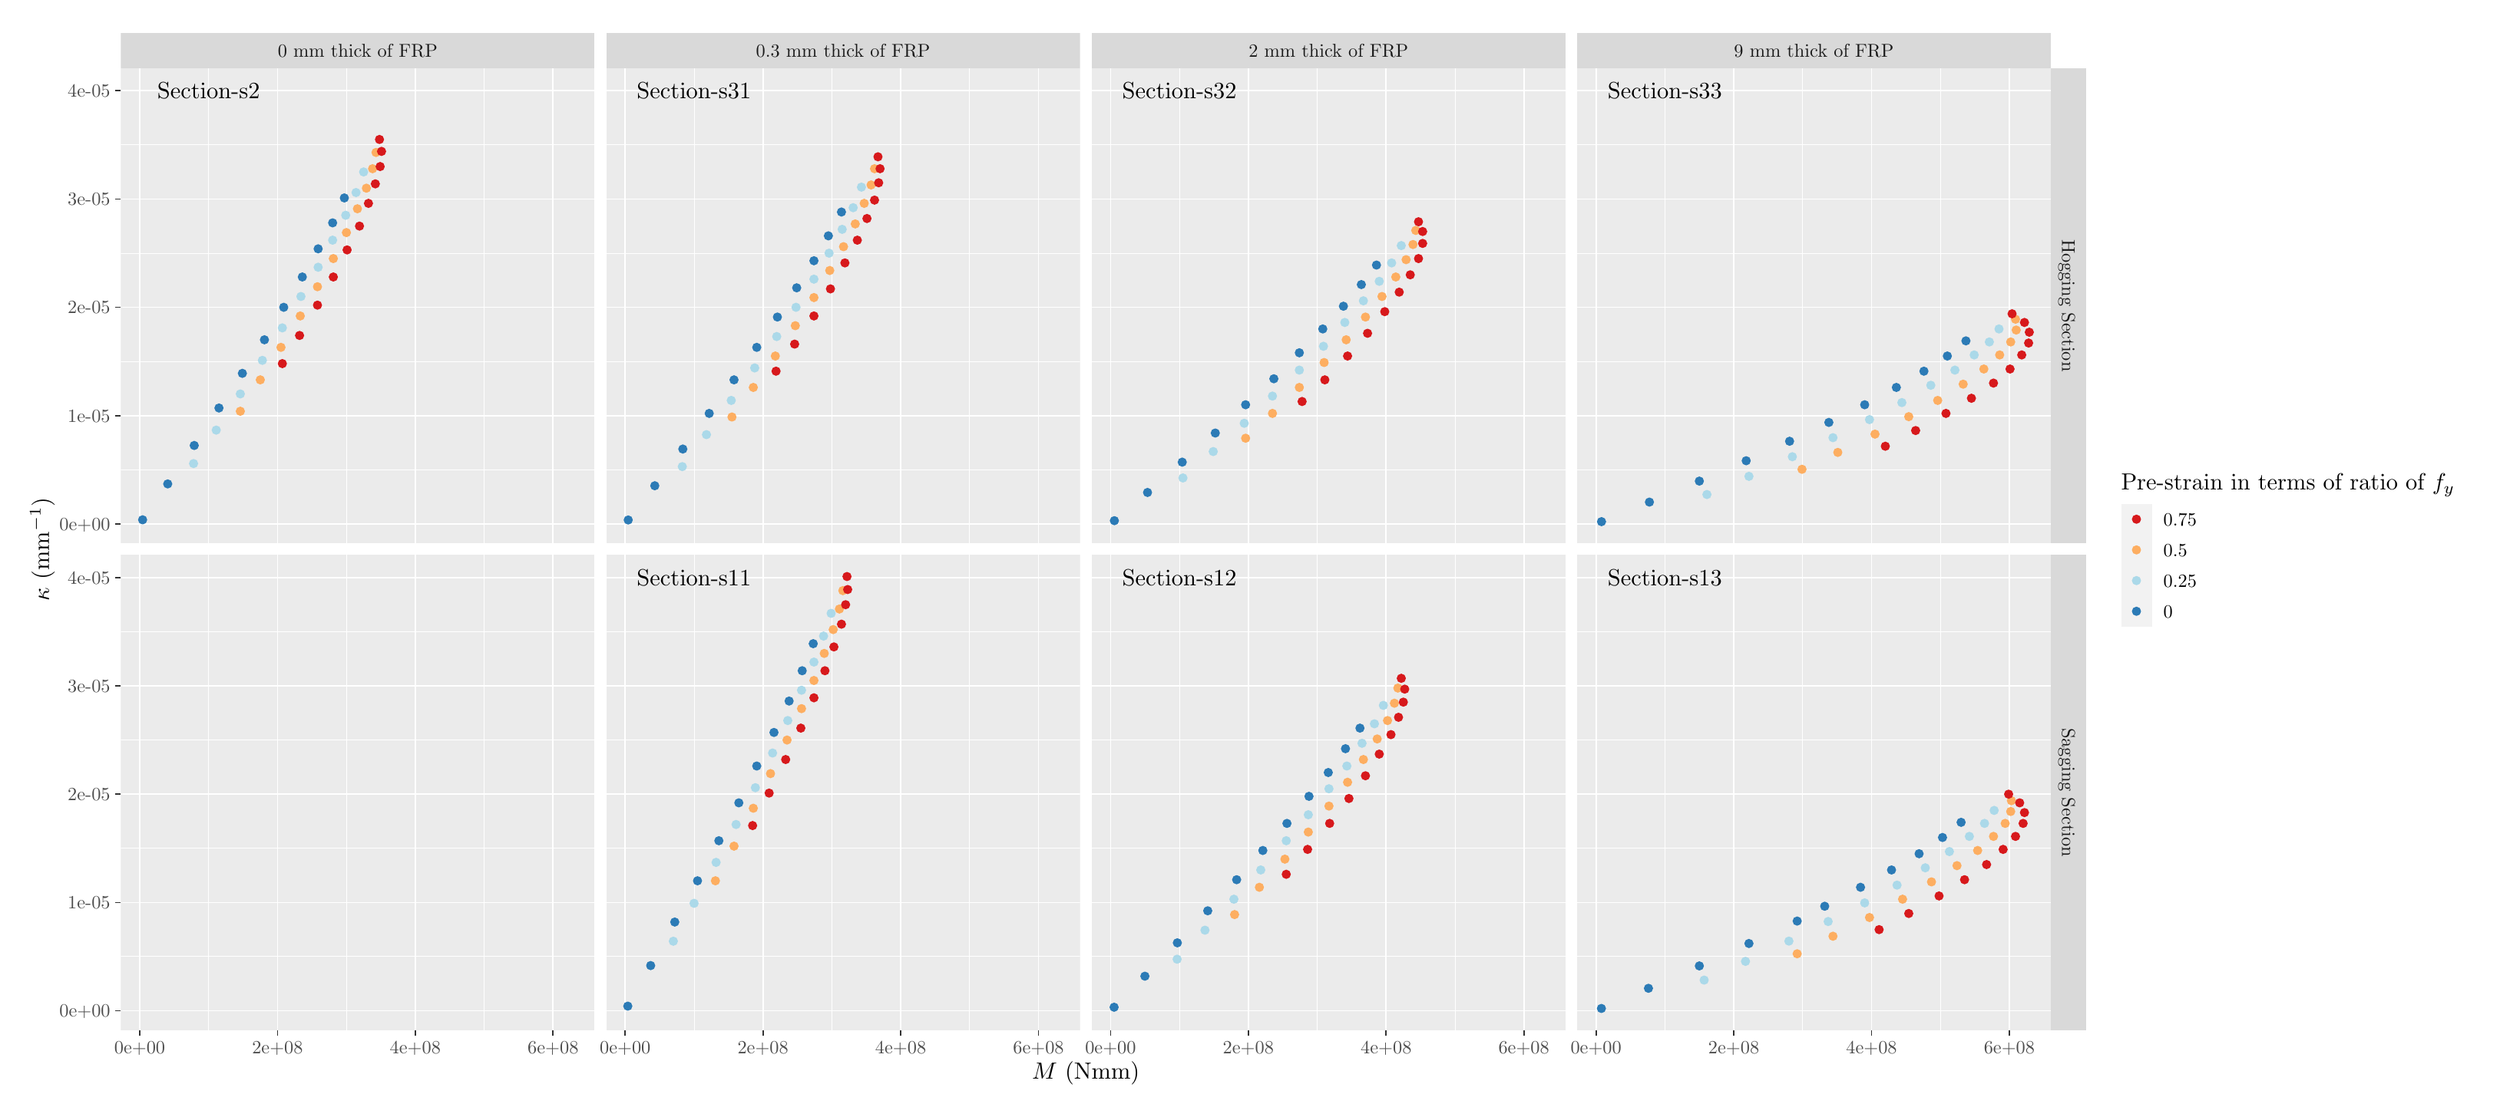
\begin{tikzpicture}[x=1pt,y=1pt]
\definecolor{fillColor}{RGB}{255,255,255}
\path[use as bounding box,fill=fillColor,fill opacity=0.00] (0,0) rectangle (1156.32,505.89);
\begin{scope}
\path[clip] (  0.00,  0.00) rectangle (1156.32,505.89);
\definecolor{drawColor}{RGB}{255,255,255}
\definecolor{fillColor}{RGB}{255,255,255}

\path[draw=drawColor,line width= 0.6pt,line join=round,line cap=round,fill=fillColor] (  0.00,  0.00) rectangle (1156.32,505.89);
\end{scope}
\begin{scope}
\path[clip] ( 46.86,260.00) rectangle (269.81,483.82);
\definecolor{fillColor}{gray}{0.92}

\path[fill=fillColor] ( 46.86,260.00) rectangle (269.81,483.82);
\definecolor{drawColor}{RGB}{255,255,255}

\path[draw=drawColor,line width= 0.3pt,line join=round] ( 46.86,294.64) --
	(269.81,294.64);

\path[draw=drawColor,line width= 0.3pt,line join=round] ( 46.86,345.64) --
	(269.81,345.64);

\path[draw=drawColor,line width= 0.3pt,line join=round] ( 46.86,396.64) --
	(269.81,396.64);

\path[draw=drawColor,line width= 0.3pt,line join=round] ( 46.86,447.64) --
	(269.81,447.64);

\path[draw=drawColor,line width= 0.3pt,line join=round] ( 88.19,260.00) --
	( 88.19,483.82);

\path[draw=drawColor,line width= 0.3pt,line join=round] (153.03,260.00) --
	(153.03,483.82);

\path[draw=drawColor,line width= 0.3pt,line join=round] (217.86,260.00) --
	(217.86,483.82);

\path[draw=drawColor,line width= 0.6pt,line join=round] ( 46.86,269.14) --
	(269.81,269.14);

\path[draw=drawColor,line width= 0.6pt,line join=round] ( 46.86,320.14) --
	(269.81,320.14);

\path[draw=drawColor,line width= 0.6pt,line join=round] ( 46.86,371.14) --
	(269.81,371.14);

\path[draw=drawColor,line width= 0.6pt,line join=round] ( 46.86,422.14) --
	(269.81,422.14);

\path[draw=drawColor,line width= 0.6pt,line join=round] ( 46.86,473.14) --
	(269.81,473.14);

\path[draw=drawColor,line width= 0.6pt,line join=round] ( 55.77,260.00) --
	( 55.77,483.82);

\path[draw=drawColor,line width= 0.6pt,line join=round] (120.61,260.00) --
	(120.61,483.82);

\path[draw=drawColor,line width= 0.6pt,line join=round] (185.44,260.00) --
	(185.44,483.82);

\path[draw=drawColor,line width= 0.6pt,line join=round] (250.28,260.00) --
	(250.28,483.82);
\definecolor{drawColor}{RGB}{44,123,182}
\definecolor{fillColor}{RGB}{44,123,182}

\path[draw=drawColor,line width= 0.4pt,line join=round,line cap=round,fill=fillColor] ( 57.12,271.05) circle (  1.96);

\path[draw=drawColor,line width= 0.4pt,line join=round,line cap=round,fill=fillColor] ( 68.93,287.95) circle (  1.96);

\path[draw=drawColor,line width= 0.4pt,line join=round,line cap=round,fill=fillColor] ( 81.41,306.06) circle (  1.96);

\path[draw=drawColor,line width= 0.4pt,line join=round,line cap=round,fill=fillColor] ( 93.05,323.71) circle (  1.96);

\path[draw=drawColor,line width= 0.4pt,line join=round,line cap=round,fill=fillColor] (104.07,340.03) circle (  1.96);

\path[draw=drawColor,line width= 0.4pt,line join=round,line cap=round,fill=fillColor] (114.45,355.84) circle (  1.96);

\path[draw=drawColor,line width= 0.4pt,line join=round,line cap=round,fill=fillColor] (123.53,371.14) circle (  1.96);

\path[draw=drawColor,line width= 0.4pt,line join=round,line cap=round,fill=fillColor] (132.28,385.42) circle (  1.96);

\path[draw=drawColor,line width= 0.4pt,line join=round,line cap=round,fill=fillColor] (139.73,398.68) circle (  1.96);

\path[draw=drawColor,line width= 0.4pt,line join=round,line cap=round,fill=fillColor] (146.54,410.92) circle (  1.96);

\path[draw=drawColor,line width= 0.4pt,line join=round,line cap=round,fill=fillColor] (152.05,422.65) circle (  1.96);
\definecolor{drawColor}{RGB}{171,217,233}
\definecolor{fillColor}{RGB}{171,217,233}

\path[draw=drawColor,line width= 0.4pt,line join=round,line cap=round,fill=fillColor] ( 81.09,297.54) circle (  1.96);

\path[draw=drawColor,line width= 0.4pt,line join=round,line cap=round,fill=fillColor] ( 91.76,313.30) circle (  1.96);

\path[draw=drawColor,line width= 0.4pt,line join=round,line cap=round,fill=fillColor] (103.10,330.34) circle (  1.96);

\path[draw=drawColor,line width= 0.4pt,line join=round,line cap=round,fill=fillColor] (113.48,346.15) circle (  1.96);

\path[draw=drawColor,line width= 0.4pt,line join=round,line cap=round,fill=fillColor] (122.88,361.45) circle (  1.96);

\path[draw=drawColor,line width= 0.4pt,line join=round,line cap=round,fill=fillColor] (131.63,376.24) circle (  1.96);

\path[draw=drawColor,line width= 0.4pt,line join=round,line cap=round,fill=fillColor] (139.73,390.01) circle (  1.96);

\path[draw=drawColor,line width= 0.4pt,line join=round,line cap=round,fill=fillColor] (146.54,402.76) circle (  1.96);

\path[draw=drawColor,line width= 0.4pt,line join=round,line cap=round,fill=fillColor] (152.70,414.49) circle (  1.96);

\path[draw=drawColor,line width= 0.4pt,line join=round,line cap=round,fill=fillColor] (157.56,425.20) circle (  1.96);

\path[draw=drawColor,line width= 0.4pt,line join=round,line cap=round,fill=fillColor] (161.13,434.89) circle (  1.96);
\definecolor{drawColor}{RGB}{253,174,97}
\definecolor{fillColor}{RGB}{253,174,97}

\path[draw=drawColor,line width= 0.4pt,line join=round,line cap=round,fill=fillColor] (103.10,322.18) circle (  1.96);

\path[draw=drawColor,line width= 0.4pt,line join=round,line cap=round,fill=fillColor] (112.50,336.97) circle (  1.96);

\path[draw=drawColor,line width= 0.4pt,line join=round,line cap=round,fill=fillColor] (122.23,352.27) circle (  1.96);

\path[draw=drawColor,line width= 0.4pt,line join=round,line cap=round,fill=fillColor] (131.31,367.06) circle (  1.96);

\path[draw=drawColor,line width= 0.4pt,line join=round,line cap=round,fill=fillColor] (139.41,380.83) circle (  1.96);

\path[draw=drawColor,line width= 0.4pt,line join=round,line cap=round,fill=fillColor] (146.87,394.09) circle (  1.96);

\path[draw=drawColor,line width= 0.4pt,line join=round,line cap=round,fill=fillColor] (153.03,406.33) circle (  1.96);

\path[draw=drawColor,line width= 0.4pt,line join=round,line cap=round,fill=fillColor] (158.21,417.55) circle (  1.96);

\path[draw=drawColor,line width= 0.4pt,line join=round,line cap=round,fill=fillColor] (162.43,427.24) circle (  1.96);

\path[draw=drawColor,line width= 0.4pt,line join=round,line cap=round,fill=fillColor] (165.34,436.42) circle (  1.96);

\path[draw=drawColor,line width= 0.4pt,line join=round,line cap=round,fill=fillColor] (166.96,444.07) circle (  1.96);
\definecolor{drawColor}{RGB}{215,25,28}
\definecolor{fillColor}{RGB}{215,25,28}

\path[draw=drawColor,line width= 0.4pt,line join=round,line cap=round,fill=fillColor] (122.88,344.62) circle (  1.96);

\path[draw=drawColor,line width= 0.4pt,line join=round,line cap=round,fill=fillColor] (130.98,357.88) circle (  1.96);

\path[draw=drawColor,line width= 0.4pt,line join=round,line cap=round,fill=fillColor] (139.41,372.16) circle (  1.96);

\path[draw=drawColor,line width= 0.4pt,line join=round,line cap=round,fill=fillColor] (146.87,385.42) circle (  1.96);

\path[draw=drawColor,line width= 0.4pt,line join=round,line cap=round,fill=fillColor] (153.35,398.17) circle (  1.96);

\path[draw=drawColor,line width= 0.4pt,line join=round,line cap=round,fill=fillColor] (159.18,409.39) circle (  1.96);

\path[draw=drawColor,line width= 0.4pt,line join=round,line cap=round,fill=fillColor] (163.40,420.10) circle (  1.96);

\path[draw=drawColor,line width= 0.4pt,line join=round,line cap=round,fill=fillColor] (166.64,429.28) circle (  1.96);

\path[draw=drawColor,line width= 0.4pt,line join=round,line cap=round,fill=fillColor] (168.91,437.44) circle (  1.96);

\path[draw=drawColor,line width= 0.4pt,line join=round,line cap=round,fill=fillColor] (169.56,444.58) circle (  1.96);

\path[draw=drawColor,line width= 0.4pt,line join=round,line cap=round,fill=fillColor] (168.59,450.19) circle (  1.96);
\definecolor{drawColor}{RGB}{0,0,0}

\node[text=drawColor,anchor=base,inner sep=0pt, outer sep=0pt, scale=  1.10] at ( 88.19,469.33) {Section-s2};
\end{scope}
\begin{scope}
\path[clip] ( 46.86, 30.69) rectangle (269.81,254.50);
\definecolor{fillColor}{gray}{0.92}

\path[fill=fillColor] ( 46.86, 30.69) rectangle (269.81,254.50);
\definecolor{drawColor}{RGB}{255,255,255}

\path[draw=drawColor,line width= 0.3pt,line join=round] ( 46.86, 65.32) --
	(269.81, 65.32);

\path[draw=drawColor,line width= 0.3pt,line join=round] ( 46.86,116.32) --
	(269.81,116.32);

\path[draw=drawColor,line width= 0.3pt,line join=round] ( 46.86,167.32) --
	(269.81,167.32);

\path[draw=drawColor,line width= 0.3pt,line join=round] ( 46.86,218.32) --
	(269.81,218.32);

\path[draw=drawColor,line width= 0.3pt,line join=round] ( 88.19, 30.69) --
	( 88.19,254.50);

\path[draw=drawColor,line width= 0.3pt,line join=round] (153.03, 30.69) --
	(153.03,254.50);

\path[draw=drawColor,line width= 0.3pt,line join=round] (217.86, 30.69) --
	(217.86,254.50);

\path[draw=drawColor,line width= 0.6pt,line join=round] ( 46.86, 39.82) --
	(269.81, 39.82);

\path[draw=drawColor,line width= 0.6pt,line join=round] ( 46.86, 90.82) --
	(269.81, 90.82);

\path[draw=drawColor,line width= 0.6pt,line join=round] ( 46.86,141.82) --
	(269.81,141.82);

\path[draw=drawColor,line width= 0.6pt,line join=round] ( 46.86,192.82) --
	(269.81,192.82);

\path[draw=drawColor,line width= 0.6pt,line join=round] ( 46.86,243.82) --
	(269.81,243.82);

\path[draw=drawColor,line width= 0.6pt,line join=round] ( 55.77, 30.69) --
	( 55.77,254.50);

\path[draw=drawColor,line width= 0.6pt,line join=round] (120.61, 30.69) --
	(120.61,254.50);

\path[draw=drawColor,line width= 0.6pt,line join=round] (185.44, 30.69) --
	(185.44,254.50);

\path[draw=drawColor,line width= 0.6pt,line join=round] (250.28, 30.69) --
	(250.28,254.50);
\end{scope}
\begin{scope}
\path[clip] (275.31,260.00) rectangle (498.26,483.82);
\definecolor{fillColor}{gray}{0.92}

\path[fill=fillColor] (275.31,260.00) rectangle (498.26,483.82);
\definecolor{drawColor}{RGB}{255,255,255}

\path[draw=drawColor,line width= 0.3pt,line join=round] (275.31,294.64) --
	(498.26,294.64);

\path[draw=drawColor,line width= 0.3pt,line join=round] (275.31,345.64) --
	(498.26,345.64);

\path[draw=drawColor,line width= 0.3pt,line join=round] (275.31,396.64) --
	(498.26,396.64);

\path[draw=drawColor,line width= 0.3pt,line join=round] (275.31,447.64) --
	(498.26,447.64);

\path[draw=drawColor,line width= 0.3pt,line join=round] (316.64,260.00) --
	(316.64,483.82);

\path[draw=drawColor,line width= 0.3pt,line join=round] (381.47,260.00) --
	(381.47,483.82);

\path[draw=drawColor,line width= 0.3pt,line join=round] (446.31,260.00) --
	(446.31,483.82);

\path[draw=drawColor,line width= 0.6pt,line join=round] (275.31,269.14) --
	(498.26,269.14);

\path[draw=drawColor,line width= 0.6pt,line join=round] (275.31,320.14) --
	(498.26,320.14);

\path[draw=drawColor,line width= 0.6pt,line join=round] (275.31,371.14) --
	(498.26,371.14);

\path[draw=drawColor,line width= 0.6pt,line join=round] (275.31,422.14) --
	(498.26,422.14);

\path[draw=drawColor,line width= 0.6pt,line join=round] (275.31,473.14) --
	(498.26,473.14);

\path[draw=drawColor,line width= 0.6pt,line join=round] (284.22,260.00) --
	(284.22,483.82);

\path[draw=drawColor,line width= 0.6pt,line join=round] (349.06,260.00) --
	(349.06,483.82);

\path[draw=drawColor,line width= 0.6pt,line join=round] (413.89,260.00) --
	(413.89,483.82);

\path[draw=drawColor,line width= 0.6pt,line join=round] (478.73,260.00) --
	(478.73,483.82);
\definecolor{drawColor}{RGB}{44,123,182}
\definecolor{fillColor}{RGB}{44,123,182}

\path[draw=drawColor,line width= 0.4pt,line join=round,line cap=round,fill=fillColor] (285.65,270.96) circle (  1.96);

\path[draw=drawColor,line width= 0.4pt,line join=round,line cap=round,fill=fillColor] (298.16,287.09) circle (  1.96);

\path[draw=drawColor,line width= 0.4pt,line join=round,line cap=round,fill=fillColor] (311.35,304.38) circle (  1.96);

\path[draw=drawColor,line width= 0.4pt,line join=round,line cap=round,fill=fillColor] (323.77,321.16) circle (  1.96);

\path[draw=drawColor,line width= 0.4pt,line join=round,line cap=round,fill=fillColor] (335.44,336.97) circle (  1.96);

\path[draw=drawColor,line width= 0.4pt,line join=round,line cap=round,fill=fillColor] (346.14,352.27) circle (  1.96);

\path[draw=drawColor,line width= 0.4pt,line join=round,line cap=round,fill=fillColor] (355.86,366.55) circle (  1.96);

\path[draw=drawColor,line width= 0.4pt,line join=round,line cap=round,fill=fillColor] (364.94,380.32) circle (  1.96);

\path[draw=drawColor,line width= 0.4pt,line join=round,line cap=round,fill=fillColor] (373.05,393.07) circle (  1.96);

\path[draw=drawColor,line width= 0.4pt,line join=round,line cap=round,fill=fillColor] (379.85,404.80) circle (  1.96);

\path[draw=drawColor,line width= 0.4pt,line join=round,line cap=round,fill=fillColor] (386.01,416.02) circle (  1.96);
\definecolor{drawColor}{RGB}{171,217,233}
\definecolor{fillColor}{RGB}{171,217,233}

\path[draw=drawColor,line width= 0.4pt,line join=round,line cap=round,fill=fillColor] (311.10,296.11) circle (  1.96);

\path[draw=drawColor,line width= 0.4pt,line join=round,line cap=round,fill=fillColor] (322.47,311.16) circle (  1.96);

\path[draw=drawColor,line width= 0.4pt,line join=round,line cap=round,fill=fillColor] (334.14,327.28) circle (  1.96);

\path[draw=drawColor,line width= 0.4pt,line join=round,line cap=round,fill=fillColor] (345.17,342.58) circle (  1.96);

\path[draw=drawColor,line width= 0.4pt,line join=round,line cap=round,fill=fillColor] (355.54,357.37) circle (  1.96);

\path[draw=drawColor,line width= 0.4pt,line join=round,line cap=round,fill=fillColor] (364.62,371.14) circle (  1.96);

\path[draw=drawColor,line width= 0.4pt,line join=round,line cap=round,fill=fillColor] (373.05,384.40) circle (  1.96);

\path[draw=drawColor,line width= 0.4pt,line join=round,line cap=round,fill=fillColor] (380.18,396.64) circle (  1.96);

\path[draw=drawColor,line width= 0.4pt,line join=round,line cap=round,fill=fillColor] (386.34,407.86) circle (  1.96);

\path[draw=drawColor,line width= 0.4pt,line join=round,line cap=round,fill=fillColor] (391.52,418.06) circle (  1.96);

\path[draw=drawColor,line width= 0.4pt,line join=round,line cap=round,fill=fillColor] (395.41,427.75) circle (  1.96);
\definecolor{drawColor}{RGB}{253,174,97}
\definecolor{fillColor}{RGB}{253,174,97}

\path[draw=drawColor,line width= 0.4pt,line join=round,line cap=round,fill=fillColor] (334.47,319.47) circle (  1.96);

\path[draw=drawColor,line width= 0.4pt,line join=round,line cap=round,fill=fillColor] (344.52,333.40) circle (  1.96);

\path[draw=drawColor,line width= 0.4pt,line join=round,line cap=round,fill=fillColor] (354.89,348.19) circle (  1.96);

\path[draw=drawColor,line width= 0.4pt,line join=round,line cap=round,fill=fillColor] (364.29,362.47) circle (  1.96);

\path[draw=drawColor,line width= 0.4pt,line join=round,line cap=round,fill=fillColor] (373.05,375.73) circle (  1.96);

\path[draw=drawColor,line width= 0.4pt,line join=round,line cap=round,fill=fillColor] (380.50,388.48) circle (  1.96);

\path[draw=drawColor,line width= 0.4pt,line join=round,line cap=round,fill=fillColor] (386.98,399.70) circle (  1.96);

\path[draw=drawColor,line width= 0.4pt,line join=round,line cap=round,fill=fillColor] (392.50,410.41) circle (  1.96);

\path[draw=drawColor,line width= 0.4pt,line join=round,line cap=round,fill=fillColor] (396.71,420.10) circle (  1.96);

\path[draw=drawColor,line width= 0.4pt,line join=round,line cap=round,fill=fillColor] (399.95,428.77) circle (  1.96);

\path[draw=drawColor,line width= 0.4pt,line join=round,line cap=round,fill=fillColor] (401.57,436.42) circle (  1.96);
\definecolor{drawColor}{RGB}{215,25,28}
\definecolor{fillColor}{RGB}{215,25,28}

\path[draw=drawColor,line width= 0.4pt,line join=round,line cap=round,fill=fillColor] (355.22,341.05) circle (  1.96);

\path[draw=drawColor,line width= 0.4pt,line join=round,line cap=round,fill=fillColor] (363.97,353.80) circle (  1.96);

\path[draw=drawColor,line width= 0.4pt,line join=round,line cap=round,fill=fillColor] (373.05,367.06) circle (  1.96);

\path[draw=drawColor,line width= 0.4pt,line join=round,line cap=round,fill=fillColor] (380.83,379.81) circle (  1.96);

\path[draw=drawColor,line width= 0.4pt,line join=round,line cap=round,fill=fillColor] (387.63,392.05) circle (  1.96);

\path[draw=drawColor,line width= 0.4pt,line join=round,line cap=round,fill=fillColor] (393.47,402.76) circle (  1.96);

\path[draw=drawColor,line width= 0.4pt,line join=round,line cap=round,fill=fillColor] (398.01,412.96) circle (  1.96);

\path[draw=drawColor,line width= 0.4pt,line join=round,line cap=round,fill=fillColor] (401.57,421.63) circle (  1.96);

\path[draw=drawColor,line width= 0.4pt,line join=round,line cap=round,fill=fillColor] (403.52,429.79) circle (  1.96);

\path[draw=drawColor,line width= 0.4pt,line join=round,line cap=round,fill=fillColor] (404.17,436.42) circle (  1.96);

\path[draw=drawColor,line width= 0.4pt,line join=round,line cap=round,fill=fillColor] (403.19,442.03) circle (  1.96);
\definecolor{drawColor}{RGB}{0,0,0}

\node[text=drawColor,anchor=base,inner sep=0pt, outer sep=0pt, scale=  1.10] at (316.64,469.33) {Section-s31};
\end{scope}
\begin{scope}
\path[clip] (275.31, 30.69) rectangle (498.26,254.50);
\definecolor{fillColor}{gray}{0.92}

\path[fill=fillColor] (275.31, 30.69) rectangle (498.26,254.50);
\definecolor{drawColor}{RGB}{255,255,255}

\path[draw=drawColor,line width= 0.3pt,line join=round] (275.31, 65.32) --
	(498.26, 65.32);

\path[draw=drawColor,line width= 0.3pt,line join=round] (275.31,116.32) --
	(498.26,116.32);

\path[draw=drawColor,line width= 0.3pt,line join=round] (275.31,167.32) --
	(498.26,167.32);

\path[draw=drawColor,line width= 0.3pt,line join=round] (275.31,218.32) --
	(498.26,218.32);

\path[draw=drawColor,line width= 0.3pt,line join=round] (316.64, 30.69) --
	(316.64,254.50);

\path[draw=drawColor,line width= 0.3pt,line join=round] (381.47, 30.69) --
	(381.47,254.50);

\path[draw=drawColor,line width= 0.3pt,line join=round] (446.31, 30.69) --
	(446.31,254.50);

\path[draw=drawColor,line width= 0.6pt,line join=round] (275.31, 39.82) --
	(498.26, 39.82);

\path[draw=drawColor,line width= 0.6pt,line join=round] (275.31, 90.82) --
	(498.26, 90.82);

\path[draw=drawColor,line width= 0.6pt,line join=round] (275.31,141.82) --
	(498.26,141.82);

\path[draw=drawColor,line width= 0.6pt,line join=round] (275.31,192.82) --
	(498.26,192.82);

\path[draw=drawColor,line width= 0.6pt,line join=round] (275.31,243.82) --
	(498.26,243.82);

\path[draw=drawColor,line width= 0.6pt,line join=round] (284.22, 30.69) --
	(284.22,254.50);

\path[draw=drawColor,line width= 0.6pt,line join=round] (349.06, 30.69) --
	(349.06,254.50);

\path[draw=drawColor,line width= 0.6pt,line join=round] (413.89, 30.69) --
	(413.89,254.50);

\path[draw=drawColor,line width= 0.6pt,line join=round] (478.73, 30.69) --
	(478.73,254.50);
\definecolor{drawColor}{RGB}{44,123,182}
\definecolor{fillColor}{RGB}{44,123,182}

\path[draw=drawColor,line width= 0.4pt,line join=round,line cap=round,fill=fillColor] (285.45, 41.98) circle (  1.96);

\path[draw=drawColor,line width= 0.4pt,line join=round,line cap=round,fill=fillColor] (296.22, 61.09) circle (  1.96);

\path[draw=drawColor,line width= 0.4pt,line join=round,line cap=round,fill=fillColor] (307.56, 81.59) circle (  1.96);

\path[draw=drawColor,line width= 0.4pt,line join=round,line cap=round,fill=fillColor] (318.26,101.02) circle (  1.96);

\path[draw=drawColor,line width= 0.4pt,line join=round,line cap=round,fill=fillColor] (328.31,119.89) circle (  1.96);

\path[draw=drawColor,line width= 0.4pt,line join=round,line cap=round,fill=fillColor] (337.71,137.74) circle (  1.96);

\path[draw=drawColor,line width= 0.4pt,line join=round,line cap=round,fill=fillColor] (346.14,155.08) circle (  1.96);

\path[draw=drawColor,line width= 0.4pt,line join=round,line cap=round,fill=fillColor] (354.24,170.89) circle (  1.96);

\path[draw=drawColor,line width= 0.4pt,line join=round,line cap=round,fill=fillColor] (361.37,185.68) circle (  1.96);

\path[draw=drawColor,line width= 0.4pt,line join=round,line cap=round,fill=fillColor] (367.53,199.96) circle (  1.96);

\path[draw=drawColor,line width= 0.4pt,line join=round,line cap=round,fill=fillColor] (372.72,212.71) circle (  1.96);
\definecolor{drawColor}{RGB}{171,217,233}
\definecolor{fillColor}{RGB}{171,217,233}

\path[draw=drawColor,line width= 0.4pt,line join=round,line cap=round,fill=fillColor] (306.88, 72.56) circle (  1.96);

\path[draw=drawColor,line width= 0.4pt,line join=round,line cap=round,fill=fillColor] (316.64, 90.41) circle (  1.96);

\path[draw=drawColor,line width= 0.4pt,line join=round,line cap=round,fill=fillColor] (327.01,109.69) circle (  1.96);

\path[draw=drawColor,line width= 0.4pt,line join=round,line cap=round,fill=fillColor] (336.41,127.54) circle (  1.96);

\path[draw=drawColor,line width= 0.4pt,line join=round,line cap=round,fill=fillColor] (345.49,144.88) circle (  1.96);

\path[draw=drawColor,line width= 0.4pt,line join=round,line cap=round,fill=fillColor] (353.59,161.20) circle (  1.96);

\path[draw=drawColor,line width= 0.4pt,line join=round,line cap=round,fill=fillColor] (360.73,176.50) circle (  1.96);

\path[draw=drawColor,line width= 0.4pt,line join=round,line cap=round,fill=fillColor] (367.21,190.78) circle (  1.96);

\path[draw=drawColor,line width= 0.4pt,line join=round,line cap=round,fill=fillColor] (373.05,204.04) circle (  1.96);

\path[draw=drawColor,line width= 0.4pt,line join=round,line cap=round,fill=fillColor] (377.58,216.28) circle (  1.96);

\path[draw=drawColor,line width= 0.4pt,line join=round,line cap=round,fill=fillColor] (381.15,226.99) circle (  1.96);
\definecolor{drawColor}{RGB}{253,174,97}
\definecolor{fillColor}{RGB}{253,174,97}

\path[draw=drawColor,line width= 0.4pt,line join=round,line cap=round,fill=fillColor] (326.69,101.02) circle (  1.96);

\path[draw=drawColor,line width= 0.4pt,line join=round,line cap=round,fill=fillColor] (335.44,117.34) circle (  1.96);

\path[draw=drawColor,line width= 0.4pt,line join=round,line cap=round,fill=fillColor] (344.52,135.19) circle (  1.96);

\path[draw=drawColor,line width= 0.4pt,line join=round,line cap=round,fill=fillColor] (352.62,151.51) circle (  1.96);

\path[draw=drawColor,line width= 0.4pt,line join=round,line cap=round,fill=fillColor] (360.40,167.32) circle (  1.96);

\path[draw=drawColor,line width= 0.4pt,line join=round,line cap=round,fill=fillColor] (367.21,182.11) circle (  1.96);

\path[draw=drawColor,line width= 0.4pt,line join=round,line cap=round,fill=fillColor] (373.05,195.37) circle (  1.96);

\path[draw=drawColor,line width= 0.4pt,line join=round,line cap=round,fill=fillColor] (377.91,208.12) circle (  1.96);

\path[draw=drawColor,line width= 0.4pt,line join=round,line cap=round,fill=fillColor] (382.12,219.34) circle (  1.96);

\path[draw=drawColor,line width= 0.4pt,line join=round,line cap=round,fill=fillColor] (385.04,229.03) circle (  1.96);

\path[draw=drawColor,line width= 0.4pt,line join=round,line cap=round,fill=fillColor] (386.66,237.70) circle (  1.96);
\definecolor{drawColor}{RGB}{215,25,28}
\definecolor{fillColor}{RGB}{215,25,28}

\path[draw=drawColor,line width= 0.4pt,line join=round,line cap=round,fill=fillColor] (344.19,127.03) circle (  1.96);

\path[draw=drawColor,line width= 0.4pt,line join=round,line cap=round,fill=fillColor] (351.97,142.33) circle (  1.96);

\path[draw=drawColor,line width= 0.4pt,line join=round,line cap=round,fill=fillColor] (359.75,158.14) circle (  1.96);

\path[draw=drawColor,line width= 0.4pt,line join=round,line cap=round,fill=fillColor] (366.89,172.93) circle (  1.96);

\path[draw=drawColor,line width= 0.4pt,line join=round,line cap=round,fill=fillColor] (373.05,187.21) circle (  1.96);

\path[draw=drawColor,line width= 0.4pt,line join=round,line cap=round,fill=fillColor] (378.23,199.96) circle (  1.96);

\path[draw=drawColor,line width= 0.4pt,line join=round,line cap=round,fill=fillColor] (382.45,211.18) circle (  1.96);

\path[draw=drawColor,line width= 0.4pt,line join=round,line cap=round,fill=fillColor] (386.01,221.89) circle (  1.96);

\path[draw=drawColor,line width= 0.4pt,line join=round,line cap=round,fill=fillColor] (387.96,231.07) circle (  1.96);

\path[draw=drawColor,line width= 0.4pt,line join=round,line cap=round,fill=fillColor] (388.93,238.21) circle (  1.96);

\path[draw=drawColor,line width= 0.4pt,line join=round,line cap=round,fill=fillColor] (388.61,244.33) circle (  1.96);
\definecolor{drawColor}{RGB}{0,0,0}

\node[text=drawColor,anchor=base,inner sep=0pt, outer sep=0pt, scale=  1.10] at (316.64,240.02) {Section-s11};
\end{scope}
\begin{scope}
\path[clip] (503.76,260.00) rectangle (726.71,483.82);
\definecolor{fillColor}{gray}{0.92}

\path[fill=fillColor] (503.76,260.00) rectangle (726.71,483.82);
\definecolor{drawColor}{RGB}{255,255,255}

\path[draw=drawColor,line width= 0.3pt,line join=round] (503.76,294.64) --
	(726.71,294.64);

\path[draw=drawColor,line width= 0.3pt,line join=round] (503.76,345.64) --
	(726.71,345.64);

\path[draw=drawColor,line width= 0.3pt,line join=round] (503.76,396.64) --
	(726.71,396.64);

\path[draw=drawColor,line width= 0.3pt,line join=round] (503.76,447.64) --
	(726.71,447.64);

\path[draw=drawColor,line width= 0.3pt,line join=round] (545.09,260.00) --
	(545.09,483.82);

\path[draw=drawColor,line width= 0.3pt,line join=round] (609.92,260.00) --
	(609.92,483.82);

\path[draw=drawColor,line width= 0.3pt,line join=round] (674.76,260.00) --
	(674.76,483.82);

\path[draw=drawColor,line width= 0.6pt,line join=round] (503.76,269.14) --
	(726.71,269.14);

\path[draw=drawColor,line width= 0.6pt,line join=round] (503.76,320.14) --
	(726.71,320.14);

\path[draw=drawColor,line width= 0.6pt,line join=round] (503.76,371.14) --
	(726.71,371.14);

\path[draw=drawColor,line width= 0.6pt,line join=round] (503.76,422.14) --
	(726.71,422.14);

\path[draw=drawColor,line width= 0.6pt,line join=round] (503.76,473.14) --
	(726.71,473.14);

\path[draw=drawColor,line width= 0.6pt,line join=round] (512.67,260.00) --
	(512.67,483.82);

\path[draw=drawColor,line width= 0.6pt,line join=round] (577.50,260.00) --
	(577.50,483.82);

\path[draw=drawColor,line width= 0.6pt,line join=round] (642.34,260.00) --
	(642.34,483.82);

\path[draw=drawColor,line width= 0.6pt,line join=round] (707.17,260.00) --
	(707.17,483.82);
\definecolor{drawColor}{RGB}{44,123,182}
\definecolor{fillColor}{RGB}{44,123,182}

\path[draw=drawColor,line width= 0.4pt,line join=round,line cap=round,fill=fillColor] (514.45,270.64) circle (  1.96);

\path[draw=drawColor,line width= 0.4pt,line join=round,line cap=round,fill=fillColor] (530.05,283.93) circle (  1.96);

\path[draw=drawColor,line width= 0.4pt,line join=round,line cap=round,fill=fillColor] (546.38,298.21) circle (  1.96);

\path[draw=drawColor,line width= 0.4pt,line join=round,line cap=round,fill=fillColor] (561.94,311.92) circle (  1.96);

\path[draw=drawColor,line width= 0.4pt,line join=round,line cap=round,fill=fillColor] (576.21,325.24) circle (  1.96);

\path[draw=drawColor,line width= 0.4pt,line join=round,line cap=round,fill=fillColor] (589.50,337.48) circle (  1.96);

\path[draw=drawColor,line width= 0.4pt,line join=round,line cap=round,fill=fillColor] (601.49,349.72) circle (  1.96);

\path[draw=drawColor,line width= 0.4pt,line join=round,line cap=round,fill=fillColor] (612.52,360.94) circle (  1.96);

\path[draw=drawColor,line width= 0.4pt,line join=round,line cap=round,fill=fillColor] (622.24,371.65) circle (  1.96);

\path[draw=drawColor,line width= 0.4pt,line join=round,line cap=round,fill=fillColor] (630.67,381.85) circle (  1.96);

\path[draw=drawColor,line width= 0.4pt,line join=round,line cap=round,fill=fillColor] (637.80,391.03) circle (  1.96);
\definecolor{drawColor}{RGB}{171,217,233}
\definecolor{fillColor}{RGB}{171,217,233}

\path[draw=drawColor,line width= 0.4pt,line join=round,line cap=round,fill=fillColor] (546.71,290.76) circle (  1.96);

\path[draw=drawColor,line width= 0.4pt,line join=round,line cap=round,fill=fillColor] (560.97,303.20) circle (  1.96);

\path[draw=drawColor,line width= 0.4pt,line join=round,line cap=round,fill=fillColor] (575.56,316.51) circle (  1.96);

\path[draw=drawColor,line width= 0.4pt,line join=round,line cap=round,fill=fillColor] (588.85,329.32) circle (  1.96);

\path[draw=drawColor,line width= 0.4pt,line join=round,line cap=round,fill=fillColor] (601.49,341.56) circle (  1.96);

\path[draw=drawColor,line width= 0.4pt,line join=round,line cap=round,fill=fillColor] (612.84,352.78) circle (  1.96);

\path[draw=drawColor,line width= 0.4pt,line join=round,line cap=round,fill=fillColor] (622.89,364.00) circle (  1.96);

\path[draw=drawColor,line width= 0.4pt,line join=round,line cap=round,fill=fillColor] (631.64,374.20) circle (  1.96);

\path[draw=drawColor,line width= 0.4pt,line join=round,line cap=round,fill=fillColor] (639.10,383.38) circle (  1.96);

\path[draw=drawColor,line width= 0.4pt,line join=round,line cap=round,fill=fillColor] (644.93,392.05) circle (  1.96);

\path[draw=drawColor,line width= 0.4pt,line join=round,line cap=round,fill=fillColor] (649.47,400.21) circle (  1.96);
\definecolor{drawColor}{RGB}{253,174,97}
\definecolor{fillColor}{RGB}{253,174,97}

\path[draw=drawColor,line width= 0.4pt,line join=round,line cap=round,fill=fillColor] (576.21,309.48) circle (  1.96);

\path[draw=drawColor,line width= 0.4pt,line join=round,line cap=round,fill=fillColor] (588.85,321.16) circle (  1.96);

\path[draw=drawColor,line width= 0.4pt,line join=round,line cap=round,fill=fillColor] (601.49,333.40) circle (  1.96);

\path[draw=drawColor,line width= 0.4pt,line join=round,line cap=round,fill=fillColor] (613.16,345.13) circle (  1.96);

\path[draw=drawColor,line width= 0.4pt,line join=round,line cap=round,fill=fillColor] (623.54,355.84) circle (  1.96);

\path[draw=drawColor,line width= 0.4pt,line join=round,line cap=round,fill=fillColor] (632.61,366.55) circle (  1.96);

\path[draw=drawColor,line width= 0.4pt,line join=round,line cap=round,fill=fillColor] (640.39,376.24) circle (  1.96);

\path[draw=drawColor,line width= 0.4pt,line join=round,line cap=round,fill=fillColor] (646.88,385.42) circle (  1.96);

\path[draw=drawColor,line width= 0.4pt,line join=round,line cap=round,fill=fillColor] (651.74,393.58) circle (  1.96);

\path[draw=drawColor,line width= 0.4pt,line join=round,line cap=round,fill=fillColor] (654.98,400.72) circle (  1.96);

\path[draw=drawColor,line width= 0.4pt,line join=round,line cap=round,fill=fillColor] (656.28,407.35) circle (  1.96);
\definecolor{drawColor}{RGB}{215,25,28}
\definecolor{fillColor}{RGB}{215,25,28}

\path[draw=drawColor,line width= 0.4pt,line join=round,line cap=round,fill=fillColor] (602.79,326.77) circle (  1.96);

\path[draw=drawColor,line width= 0.4pt,line join=round,line cap=round,fill=fillColor] (613.49,336.97) circle (  1.96);

\path[draw=drawColor,line width= 0.4pt,line join=round,line cap=round,fill=fillColor] (624.19,348.19) circle (  1.96);

\path[draw=drawColor,line width= 0.4pt,line join=round,line cap=round,fill=fillColor] (633.59,358.90) circle (  1.96);

\path[draw=drawColor,line width= 0.4pt,line join=round,line cap=round,fill=fillColor] (641.69,369.10) circle (  1.96);

\path[draw=drawColor,line width= 0.4pt,line join=round,line cap=round,fill=fillColor] (648.50,378.28) circle (  1.96);

\path[draw=drawColor,line width= 0.4pt,line join=round,line cap=round,fill=fillColor] (653.69,386.44) circle (  1.96);

\path[draw=drawColor,line width= 0.4pt,line join=round,line cap=round,fill=fillColor] (657.58,394.09) circle (  1.96);

\path[draw=drawColor,line width= 0.4pt,line join=round,line cap=round,fill=fillColor] (659.52,401.23) circle (  1.96);

\path[draw=drawColor,line width= 0.4pt,line join=round,line cap=round,fill=fillColor] (659.52,406.84) circle (  1.96);

\path[draw=drawColor,line width= 0.4pt,line join=round,line cap=round,fill=fillColor] (657.58,411.43) circle (  1.96);
\definecolor{drawColor}{RGB}{0,0,0}

\node[text=drawColor,anchor=base,inner sep=0pt, outer sep=0pt, scale=  1.10] at (545.09,469.33) {Section-s32};
\end{scope}
\begin{scope}
\path[clip] (503.76, 30.69) rectangle (726.71,254.50);
\definecolor{fillColor}{gray}{0.92}

\path[fill=fillColor] (503.76, 30.69) rectangle (726.71,254.50);
\definecolor{drawColor}{RGB}{255,255,255}

\path[draw=drawColor,line width= 0.3pt,line join=round] (503.76, 65.32) --
	(726.71, 65.32);

\path[draw=drawColor,line width= 0.3pt,line join=round] (503.76,116.32) --
	(726.71,116.32);

\path[draw=drawColor,line width= 0.3pt,line join=round] (503.76,167.32) --
	(726.71,167.32);

\path[draw=drawColor,line width= 0.3pt,line join=round] (503.76,218.32) --
	(726.71,218.32);

\path[draw=drawColor,line width= 0.3pt,line join=round] (545.09, 30.69) --
	(545.09,254.50);

\path[draw=drawColor,line width= 0.3pt,line join=round] (609.92, 30.69) --
	(609.92,254.50);

\path[draw=drawColor,line width= 0.3pt,line join=round] (674.76, 30.69) --
	(674.76,254.50);

\path[draw=drawColor,line width= 0.6pt,line join=round] (503.76, 39.82) --
	(726.71, 39.82);

\path[draw=drawColor,line width= 0.6pt,line join=round] (503.76, 90.82) --
	(726.71, 90.82);

\path[draw=drawColor,line width= 0.6pt,line join=round] (503.76,141.82) --
	(726.71,141.82);

\path[draw=drawColor,line width= 0.6pt,line join=round] (503.76,192.82) --
	(726.71,192.82);

\path[draw=drawColor,line width= 0.6pt,line join=round] (503.76,243.82) --
	(726.71,243.82);

\path[draw=drawColor,line width= 0.6pt,line join=round] (512.67, 30.69) --
	(512.67,254.50);

\path[draw=drawColor,line width= 0.6pt,line join=round] (577.50, 30.69) --
	(577.50,254.50);

\path[draw=drawColor,line width= 0.6pt,line join=round] (642.34, 30.69) --
	(642.34,254.50);

\path[draw=drawColor,line width= 0.6pt,line join=round] (707.17, 30.69) --
	(707.17,254.50);
\definecolor{drawColor}{RGB}{44,123,182}
\definecolor{fillColor}{RGB}{44,123,182}

\path[draw=drawColor,line width= 0.4pt,line join=round,line cap=round,fill=fillColor] (514.32, 41.47) circle (  1.96);

\path[draw=drawColor,line width= 0.4pt,line join=round,line cap=round,fill=fillColor] (528.81, 56.09) circle (  1.96);

\path[draw=drawColor,line width= 0.4pt,line join=round,line cap=round,fill=fillColor] (544.08, 71.80) circle (  1.96);

\path[draw=drawColor,line width= 0.4pt,line join=round,line cap=round,fill=fillColor] (558.38, 86.89) circle (  1.96);

\path[draw=drawColor,line width= 0.4pt,line join=round,line cap=round,fill=fillColor] (571.99,101.53) circle (  1.96);

\path[draw=drawColor,line width= 0.4pt,line join=round,line cap=round,fill=fillColor] (584.31,115.30) circle (  1.96);

\path[draw=drawColor,line width= 0.4pt,line join=round,line cap=round,fill=fillColor] (595.66,128.05) circle (  1.96);

\path[draw=drawColor,line width= 0.4pt,line join=round,line cap=round,fill=fillColor] (606.03,140.80) circle (  1.96);

\path[draw=drawColor,line width= 0.4pt,line join=round,line cap=round,fill=fillColor] (615.11,152.02) circle (  1.96);

\path[draw=drawColor,line width= 0.4pt,line join=round,line cap=round,fill=fillColor] (623.21,163.24) circle (  1.96);

\path[draw=drawColor,line width= 0.4pt,line join=round,line cap=round,fill=fillColor] (630.02,172.93) circle (  1.96);
\definecolor{drawColor}{RGB}{171,217,233}
\definecolor{fillColor}{RGB}{171,217,233}

\path[draw=drawColor,line width= 0.4pt,line join=round,line cap=round,fill=fillColor] (543.98, 64.09) circle (  1.96);

\path[draw=drawColor,line width= 0.4pt,line join=round,line cap=round,fill=fillColor] (557.08, 77.76) circle (  1.96);

\path[draw=drawColor,line width= 0.4pt,line join=round,line cap=round,fill=fillColor] (570.70, 92.35) circle (  1.96);

\path[draw=drawColor,line width= 0.4pt,line join=round,line cap=round,fill=fillColor] (583.34,106.12) circle (  1.96);

\path[draw=drawColor,line width= 0.4pt,line join=round,line cap=round,fill=fillColor] (595.33,119.89) circle (  1.96);

\path[draw=drawColor,line width= 0.4pt,line join=round,line cap=round,fill=fillColor] (605.71,132.13) circle (  1.96);

\path[draw=drawColor,line width= 0.4pt,line join=round,line cap=round,fill=fillColor] (615.43,144.37) circle (  1.96);

\path[draw=drawColor,line width= 0.4pt,line join=round,line cap=round,fill=fillColor] (623.86,155.08) circle (  1.96);

\path[draw=drawColor,line width= 0.4pt,line join=round,line cap=round,fill=fillColor] (630.99,165.79) circle (  1.96);

\path[draw=drawColor,line width= 0.4pt,line join=round,line cap=round,fill=fillColor] (636.83,174.97) circle (  1.96);

\path[draw=drawColor,line width= 0.4pt,line join=round,line cap=round,fill=fillColor] (641.04,183.64) circle (  1.96);
\definecolor{drawColor}{RGB}{253,174,97}
\definecolor{fillColor}{RGB}{253,174,97}

\path[draw=drawColor,line width= 0.4pt,line join=round,line cap=round,fill=fillColor] (571.02, 85.11) circle (  1.96);

\path[draw=drawColor,line width= 0.4pt,line join=round,line cap=round,fill=fillColor] (582.69, 97.96) circle (  1.96);

\path[draw=drawColor,line width= 0.4pt,line join=round,line cap=round,fill=fillColor] (594.69,111.22) circle (  1.96);

\path[draw=drawColor,line width= 0.4pt,line join=round,line cap=round,fill=fillColor] (605.71,123.97) circle (  1.96);

\path[draw=drawColor,line width= 0.4pt,line join=round,line cap=round,fill=fillColor] (615.43,136.21) circle (  1.96);

\path[draw=drawColor,line width= 0.4pt,line join=round,line cap=round,fill=fillColor] (624.19,147.43) circle (  1.96);

\path[draw=drawColor,line width= 0.4pt,line join=round,line cap=round,fill=fillColor] (631.64,158.14) circle (  1.96);

\path[draw=drawColor,line width= 0.4pt,line join=round,line cap=round,fill=fillColor] (638.13,167.83) circle (  1.96);

\path[draw=drawColor,line width= 0.4pt,line join=round,line cap=round,fill=fillColor] (642.99,176.50) circle (  1.96);

\path[draw=drawColor,line width= 0.4pt,line join=round,line cap=round,fill=fillColor] (646.23,184.66) circle (  1.96);

\path[draw=drawColor,line width= 0.4pt,line join=round,line cap=round,fill=fillColor] (647.85,191.80) circle (  1.96);
\definecolor{drawColor}{RGB}{215,25,28}
\definecolor{fillColor}{RGB}{215,25,28}

\path[draw=drawColor,line width= 0.4pt,line join=round,line cap=round,fill=fillColor] (595.33,104.08) circle (  1.96);

\path[draw=drawColor,line width= 0.4pt,line join=round,line cap=round,fill=fillColor] (605.38,115.81) circle (  1.96);

\path[draw=drawColor,line width= 0.4pt,line join=round,line cap=round,fill=fillColor] (615.76,128.05) circle (  1.96);

\path[draw=drawColor,line width= 0.4pt,line join=round,line cap=round,fill=fillColor] (624.83,139.78) circle (  1.96);

\path[draw=drawColor,line width= 0.4pt,line join=round,line cap=round,fill=fillColor] (632.61,150.49) circle (  1.96);

\path[draw=drawColor,line width= 0.4pt,line join=round,line cap=round,fill=fillColor] (639.10,160.69) circle (  1.96);

\path[draw=drawColor,line width= 0.4pt,line join=round,line cap=round,fill=fillColor] (644.61,169.87) circle (  1.96);

\path[draw=drawColor,line width= 0.4pt,line join=round,line cap=round,fill=fillColor] (648.17,178.03) circle (  1.96);

\path[draw=drawColor,line width= 0.4pt,line join=round,line cap=round,fill=fillColor] (650.44,185.17) circle (  1.96);

\path[draw=drawColor,line width= 0.4pt,line join=round,line cap=round,fill=fillColor] (651.09,191.29) circle (  1.96);

\path[draw=drawColor,line width= 0.4pt,line join=round,line cap=round,fill=fillColor] (649.47,196.39) circle (  1.96);
\definecolor{drawColor}{RGB}{0,0,0}

\node[text=drawColor,anchor=base,inner sep=0pt, outer sep=0pt, scale=  1.10] at (545.09,240.02) {Section-s12};
\end{scope}
\begin{scope}
\path[clip] (732.21,260.00) rectangle (955.16,483.82);
\definecolor{fillColor}{gray}{0.92}

\path[fill=fillColor] (732.21,260.00) rectangle (955.16,483.82);
\definecolor{drawColor}{RGB}{255,255,255}

\path[draw=drawColor,line width= 0.3pt,line join=round] (732.21,294.64) --
	(955.16,294.64);

\path[draw=drawColor,line width= 0.3pt,line join=round] (732.21,345.64) --
	(955.16,345.64);

\path[draw=drawColor,line width= 0.3pt,line join=round] (732.21,396.64) --
	(955.16,396.64);

\path[draw=drawColor,line width= 0.3pt,line join=round] (732.21,447.64) --
	(955.16,447.64);

\path[draw=drawColor,line width= 0.3pt,line join=round] (773.54,260.00) --
	(773.54,483.82);

\path[draw=drawColor,line width= 0.3pt,line join=round] (838.37,260.00) --
	(838.37,483.82);

\path[draw=drawColor,line width= 0.3pt,line join=round] (903.21,260.00) --
	(903.21,483.82);

\path[draw=drawColor,line width= 0.6pt,line join=round] (732.21,269.14) --
	(955.16,269.14);

\path[draw=drawColor,line width= 0.6pt,line join=round] (732.21,320.14) --
	(955.16,320.14);

\path[draw=drawColor,line width= 0.6pt,line join=round] (732.21,371.14) --
	(955.16,371.14);

\path[draw=drawColor,line width= 0.6pt,line join=round] (732.21,422.14) --
	(955.16,422.14);

\path[draw=drawColor,line width= 0.6pt,line join=round] (732.21,473.14) --
	(955.16,473.14);

\path[draw=drawColor,line width= 0.6pt,line join=round] (741.12,260.00) --
	(741.12,483.82);

\path[draw=drawColor,line width= 0.6pt,line join=round] (805.95,260.00) --
	(805.95,483.82);

\path[draw=drawColor,line width= 0.6pt,line join=round] (870.79,260.00) --
	(870.79,483.82);

\path[draw=drawColor,line width= 0.6pt,line join=round] (935.62,260.00) --
	(935.62,483.82);
\definecolor{drawColor}{RGB}{44,123,182}
\definecolor{fillColor}{RGB}{44,123,182}

\path[draw=drawColor,line width= 0.4pt,line join=round,line cap=round,fill=fillColor] (743.70,270.18) circle (  1.96);

\path[draw=drawColor,line width= 0.4pt,line join=round,line cap=round,fill=fillColor] (766.24,279.39) circle (  1.96);

\path[draw=drawColor,line width= 0.4pt,line join=round,line cap=round,fill=fillColor] (789.74,289.28) circle (  1.96);

\path[draw=drawColor,line width= 0.4pt,line join=round,line cap=round,fill=fillColor] (811.79,298.87) circle (  1.96);

\path[draw=drawColor,line width= 0.4pt,line join=round,line cap=round,fill=fillColor] (832.21,308.05) circle (  1.96);

\path[draw=drawColor,line width= 0.4pt,line join=round,line cap=round,fill=fillColor] (850.69,316.92) circle (  1.96);

\path[draw=drawColor,line width= 0.4pt,line join=round,line cap=round,fill=fillColor] (867.55,325.24) circle (  1.96);

\path[draw=drawColor,line width= 0.4pt,line join=round,line cap=round,fill=fillColor] (882.46,333.40) circle (  1.96);

\path[draw=drawColor,line width= 0.4pt,line join=round,line cap=round,fill=fillColor] (895.43,341.05) circle (  1.96);

\path[draw=drawColor,line width= 0.4pt,line join=round,line cap=round,fill=fillColor] (906.45,348.19) circle (  1.96);

\path[draw=drawColor,line width= 0.4pt,line join=round,line cap=round,fill=fillColor] (915.20,355.33) circle (  1.96);
\definecolor{drawColor}{RGB}{171,217,233}
\definecolor{fillColor}{RGB}{171,217,233}

\path[draw=drawColor,line width= 0.4pt,line join=round,line cap=round,fill=fillColor] (793.31,282.96) circle (  1.96);

\path[draw=drawColor,line width= 0.4pt,line join=round,line cap=round,fill=fillColor] (813.08,291.52) circle (  1.96);

\path[draw=drawColor,line width= 0.4pt,line join=round,line cap=round,fill=fillColor] (833.51,300.76) circle (  1.96);

\path[draw=drawColor,line width= 0.4pt,line join=round,line cap=round,fill=fillColor] (852.63,309.73) circle (  1.96);

\path[draw=drawColor,line width= 0.4pt,line join=round,line cap=round,fill=fillColor] (869.82,318.25) circle (  1.96);

\path[draw=drawColor,line width= 0.4pt,line join=round,line cap=round,fill=fillColor] (885.05,326.26) circle (  1.96);

\path[draw=drawColor,line width= 0.4pt,line join=round,line cap=round,fill=fillColor] (898.67,334.42) circle (  1.96);

\path[draw=drawColor,line width= 0.4pt,line join=round,line cap=round,fill=fillColor] (910.01,341.56) circle (  1.96);

\path[draw=drawColor,line width= 0.4pt,line join=round,line cap=round,fill=fillColor] (919.09,348.70) circle (  1.96);

\path[draw=drawColor,line width= 0.4pt,line join=round,line cap=round,fill=fillColor] (926.22,354.82) circle (  1.96);

\path[draw=drawColor,line width= 0.4pt,line join=round,line cap=round,fill=fillColor] (930.76,360.94) circle (  1.96);
\definecolor{drawColor}{RGB}{253,174,97}
\definecolor{fillColor}{RGB}{253,174,97}

\path[draw=drawColor,line width= 0.4pt,line join=round,line cap=round,fill=fillColor] (838.05,294.84) circle (  1.96);

\path[draw=drawColor,line width= 0.4pt,line join=round,line cap=round,fill=fillColor] (854.90,302.80) circle (  1.96);

\path[draw=drawColor,line width= 0.4pt,line join=round,line cap=round,fill=fillColor] (872.41,311.41) circle (  1.96);

\path[draw=drawColor,line width= 0.4pt,line join=round,line cap=round,fill=fillColor] (888.29,319.63) circle (  1.96);

\path[draw=drawColor,line width= 0.4pt,line join=round,line cap=round,fill=fillColor] (901.91,327.28) circle (  1.96);

\path[draw=drawColor,line width= 0.4pt,line join=round,line cap=round,fill=fillColor] (913.90,334.93) circle (  1.96);

\path[draw=drawColor,line width= 0.4pt,line join=round,line cap=round,fill=fillColor] (923.63,342.07) circle (  1.96);

\path[draw=drawColor,line width= 0.4pt,line join=round,line cap=round,fill=fillColor] (931.08,348.70) circle (  1.96);

\path[draw=drawColor,line width= 0.4pt,line join=round,line cap=round,fill=fillColor] (936.27,354.82) circle (  1.96);

\path[draw=drawColor,line width= 0.4pt,line join=round,line cap=round,fill=fillColor] (938.86,360.43) circle (  1.96);

\path[draw=drawColor,line width= 0.4pt,line join=round,line cap=round,fill=fillColor] (938.54,365.53) circle (  1.96);
\definecolor{drawColor}{RGB}{215,25,28}
\definecolor{fillColor}{RGB}{215,25,28}

\path[draw=drawColor,line width= 0.4pt,line join=round,line cap=round,fill=fillColor] (877.27,305.70) circle (  1.96);

\path[draw=drawColor,line width= 0.4pt,line join=round,line cap=round,fill=fillColor] (891.53,313.10) circle (  1.96);

\path[draw=drawColor,line width= 0.4pt,line join=round,line cap=round,fill=fillColor] (905.80,321.16) circle (  1.96);

\path[draw=drawColor,line width= 0.4pt,line join=round,line cap=round,fill=fillColor] (917.79,328.30) circle (  1.96);

\path[draw=drawColor,line width= 0.4pt,line join=round,line cap=round,fill=fillColor] (928.17,335.44) circle (  1.96);

\path[draw=drawColor,line width= 0.4pt,line join=round,line cap=round,fill=fillColor] (935.95,342.07) circle (  1.96);

\path[draw=drawColor,line width= 0.4pt,line join=round,line cap=round,fill=fillColor] (941.46,348.70) circle (  1.96);

\path[draw=drawColor,line width= 0.4pt,line join=round,line cap=round,fill=fillColor] (944.70,354.31) circle (  1.96);

\path[draw=drawColor,line width= 0.4pt,line join=round,line cap=round,fill=fillColor] (945.02,359.41) circle (  1.96);

\path[draw=drawColor,line width= 0.4pt,line join=round,line cap=round,fill=fillColor] (942.75,364.00) circle (  1.96);

\path[draw=drawColor,line width= 0.4pt,line join=round,line cap=round,fill=fillColor] (936.92,368.08) circle (  1.96);
\definecolor{drawColor}{RGB}{0,0,0}

\node[text=drawColor,anchor=base,inner sep=0pt, outer sep=0pt, scale=  1.10] at (773.54,469.33) {Section-s33};
\end{scope}
\begin{scope}
\path[clip] (732.21, 30.69) rectangle (955.16,254.50);
\definecolor{fillColor}{gray}{0.92}

\path[fill=fillColor] (732.21, 30.69) rectangle (955.16,254.50);
\definecolor{drawColor}{RGB}{255,255,255}

\path[draw=drawColor,line width= 0.3pt,line join=round] (732.21, 65.32) --
	(955.16, 65.32);

\path[draw=drawColor,line width= 0.3pt,line join=round] (732.21,116.32) --
	(955.16,116.32);

\path[draw=drawColor,line width= 0.3pt,line join=round] (732.21,167.32) --
	(955.16,167.32);

\path[draw=drawColor,line width= 0.3pt,line join=round] (732.21,218.32) --
	(955.16,218.32);

\path[draw=drawColor,line width= 0.3pt,line join=round] (773.54, 30.69) --
	(773.54,254.50);

\path[draw=drawColor,line width= 0.3pt,line join=round] (838.37, 30.69) --
	(838.37,254.50);

\path[draw=drawColor,line width= 0.3pt,line join=round] (903.21, 30.69) --
	(903.21,254.50);

\path[draw=drawColor,line width= 0.6pt,line join=round] (732.21, 39.82) --
	(955.16, 39.82);

\path[draw=drawColor,line width= 0.6pt,line join=round] (732.21, 90.82) --
	(955.16, 90.82);

\path[draw=drawColor,line width= 0.6pt,line join=round] (732.21,141.82) --
	(955.16,141.82);

\path[draw=drawColor,line width= 0.6pt,line join=round] (732.21,192.82) --
	(955.16,192.82);

\path[draw=drawColor,line width= 0.6pt,line join=round] (732.21,243.82) --
	(955.16,243.82);

\path[draw=drawColor,line width= 0.6pt,line join=round] (741.12, 30.69) --
	(741.12,254.50);

\path[draw=drawColor,line width= 0.6pt,line join=round] (805.95, 30.69) --
	(805.95,254.50);

\path[draw=drawColor,line width= 0.6pt,line join=round] (870.79, 30.69) --
	(870.79,254.50);

\path[draw=drawColor,line width= 0.6pt,line join=round] (935.62, 30.69) --
	(935.62,254.50);
\definecolor{drawColor}{RGB}{44,123,182}
\definecolor{fillColor}{RGB}{44,123,182}

\path[draw=drawColor,line width= 0.4pt,line join=round,line cap=round,fill=fillColor] (743.65, 40.89) circle (  1.96);

\path[draw=drawColor,line width= 0.4pt,line join=round,line cap=round,fill=fillColor] (765.79, 50.38) circle (  1.96);

\path[draw=drawColor,line width= 0.4pt,line join=round,line cap=round,fill=fillColor] (789.74, 60.93) circle (  1.96);

\path[draw=drawColor,line width= 0.4pt,line join=round,line cap=round,fill=fillColor] (813.08, 71.49) circle (  1.96);

\path[draw=drawColor,line width= 0.4pt,line join=round,line cap=round,fill=fillColor] (835.78, 82.05) circle (  1.96);

\path[draw=drawColor,line width= 0.4pt,line join=round,line cap=round,fill=fillColor] (848.74, 89.03) circle (  1.96);

\path[draw=drawColor,line width= 0.4pt,line join=round,line cap=round,fill=fillColor] (865.60, 97.96) circle (  1.96);

\path[draw=drawColor,line width= 0.4pt,line join=round,line cap=round,fill=fillColor] (880.19,106.12) circle (  1.96);

\path[draw=drawColor,line width= 0.4pt,line join=round,line cap=round,fill=fillColor] (893.16,113.77) circle (  1.96);

\path[draw=drawColor,line width= 0.4pt,line join=round,line cap=round,fill=fillColor] (904.18,121.42) circle (  1.96);

\path[draw=drawColor,line width= 0.4pt,line join=round,line cap=round,fill=fillColor] (912.93,128.56) circle (  1.96);
\definecolor{drawColor}{RGB}{171,217,233}
\definecolor{fillColor}{RGB}{171,217,233}

\path[draw=drawColor,line width= 0.4pt,line join=round,line cap=round,fill=fillColor] (792.01, 54.25) circle (  1.96);

\path[draw=drawColor,line width= 0.4pt,line join=round,line cap=round,fill=fillColor] (811.46, 63.07) circle (  1.96);

\path[draw=drawColor,line width= 0.4pt,line join=round,line cap=round,fill=fillColor] (831.89, 72.61) circle (  1.96);

\path[draw=drawColor,line width= 0.4pt,line join=round,line cap=round,fill=fillColor] (850.36, 81.84) circle (  1.96);

\path[draw=drawColor,line width= 0.4pt,line join=round,line cap=round,fill=fillColor] (867.55, 90.61) circle (  1.96);

\path[draw=drawColor,line width= 0.4pt,line join=round,line cap=round,fill=fillColor] (882.78, 98.98) circle (  1.96);

\path[draw=drawColor,line width= 0.4pt,line join=round,line cap=round,fill=fillColor] (896.07,107.14) circle (  1.96);

\path[draw=drawColor,line width= 0.4pt,line join=round,line cap=round,fill=fillColor] (907.42,114.79) circle (  1.96);

\path[draw=drawColor,line width= 0.4pt,line join=round,line cap=round,fill=fillColor] (916.82,121.93) circle (  1.96);

\path[draw=drawColor,line width= 0.4pt,line join=round,line cap=round,fill=fillColor] (923.95,128.05) circle (  1.96);

\path[draw=drawColor,line width= 0.4pt,line join=round,line cap=round,fill=fillColor] (928.49,134.17) circle (  1.96);
\definecolor{drawColor}{RGB}{253,174,97}
\definecolor{fillColor}{RGB}{253,174,97}

\path[draw=drawColor,line width= 0.4pt,line join=round,line cap=round,fill=fillColor] (835.78, 66.64) circle (  1.96);

\path[draw=drawColor,line width= 0.4pt,line join=round,line cap=round,fill=fillColor] (852.63, 74.91) circle (  1.96);

\path[draw=drawColor,line width= 0.4pt,line join=round,line cap=round,fill=fillColor] (869.82, 83.73) circle (  1.96);

\path[draw=drawColor,line width= 0.4pt,line join=round,line cap=round,fill=fillColor] (885.38, 92.35) circle (  1.96);

\path[draw=drawColor,line width= 0.4pt,line join=round,line cap=round,fill=fillColor] (898.99,100.51) circle (  1.96);

\path[draw=drawColor,line width= 0.4pt,line join=round,line cap=round,fill=fillColor] (910.99,108.16) circle (  1.96);

\path[draw=drawColor,line width= 0.4pt,line join=round,line cap=round,fill=fillColor] (920.71,115.30) circle (  1.96);

\path[draw=drawColor,line width= 0.4pt,line join=round,line cap=round,fill=fillColor] (928.17,121.93) circle (  1.96);

\path[draw=drawColor,line width= 0.4pt,line join=round,line cap=round,fill=fillColor] (933.68,128.05) circle (  1.96);

\path[draw=drawColor,line width= 0.4pt,line join=round,line cap=round,fill=fillColor] (936.27,133.66) circle (  1.96);

\path[draw=drawColor,line width= 0.4pt,line join=round,line cap=round,fill=fillColor] (936.60,138.76) circle (  1.96);
\definecolor{drawColor}{RGB}{215,25,28}
\definecolor{fillColor}{RGB}{215,25,28}

\path[draw=drawColor,line width= 0.4pt,line join=round,line cap=round,fill=fillColor] (874.35, 78.02) circle (  1.96);

\path[draw=drawColor,line width= 0.4pt,line join=round,line cap=round,fill=fillColor] (888.29, 85.62) circle (  1.96);

\path[draw=drawColor,line width= 0.4pt,line join=round,line cap=round,fill=fillColor] (902.56, 93.88) circle (  1.96);

\path[draw=drawColor,line width= 0.4pt,line join=round,line cap=round,fill=fillColor] (914.55,101.53) circle (  1.96);

\path[draw=drawColor,line width= 0.4pt,line join=round,line cap=round,fill=fillColor] (924.92,108.67) circle (  1.96);

\path[draw=drawColor,line width= 0.4pt,line join=round,line cap=round,fill=fillColor] (932.71,115.81) circle (  1.96);

\path[draw=drawColor,line width= 0.4pt,line join=round,line cap=round,fill=fillColor] (938.54,121.93) circle (  1.96);

\path[draw=drawColor,line width= 0.4pt,line join=round,line cap=round,fill=fillColor] (942.11,128.05) circle (  1.96);

\path[draw=drawColor,line width= 0.4pt,line join=round,line cap=round,fill=fillColor] (942.75,133.15) circle (  1.96);

\path[draw=drawColor,line width= 0.4pt,line join=round,line cap=round,fill=fillColor] (940.49,137.74) circle (  1.96);

\path[draw=drawColor,line width= 0.4pt,line join=round,line cap=round,fill=fillColor] (935.30,141.82) circle (  1.96);
\definecolor{drawColor}{RGB}{0,0,0}

\node[text=drawColor,anchor=base,inner sep=0pt, outer sep=0pt, scale=  1.10] at (773.54,240.02) {Section-s13};
\end{scope}
\begin{scope}
\path[clip] ( 46.86,483.82) rectangle (269.81,500.39);
\definecolor{fillColor}{gray}{0.85}

\path[fill=fillColor] ( 46.86,483.82) rectangle (269.81,500.39);
\definecolor{drawColor}{gray}{0.10}

\node[text=drawColor,anchor=base,inner sep=0pt, outer sep=0pt, scale=  0.88] at (158.34,489.07) {0 mm thick of FRP};
\end{scope}
\begin{scope}
\path[clip] (275.31,483.82) rectangle (498.26,500.39);
\definecolor{fillColor}{gray}{0.85}

\path[fill=fillColor] (275.31,483.82) rectangle (498.26,500.39);
\definecolor{drawColor}{gray}{0.10}

\node[text=drawColor,anchor=base,inner sep=0pt, outer sep=0pt, scale=  0.88] at (386.79,489.07) {0.3 mm thick of FRP};
\end{scope}
\begin{scope}
\path[clip] (503.76,483.82) rectangle (726.71,500.39);
\definecolor{fillColor}{gray}{0.85}

\path[fill=fillColor] (503.76,483.82) rectangle (726.71,500.39);
\definecolor{drawColor}{gray}{0.10}

\node[text=drawColor,anchor=base,inner sep=0pt, outer sep=0pt, scale=  0.88] at (615.24,489.07) {2 mm thick of FRP};
\end{scope}
\begin{scope}
\path[clip] (732.21,483.82) rectangle (955.16,500.39);
\definecolor{fillColor}{gray}{0.85}

\path[fill=fillColor] (732.21,483.82) rectangle (955.16,500.39);
\definecolor{drawColor}{gray}{0.10}

\node[text=drawColor,anchor=base,inner sep=0pt, outer sep=0pt, scale=  0.88] at (843.68,489.07) {9 mm thick of FRP};
\end{scope}
\begin{scope}
\path[clip] (955.16,260.00) rectangle (971.73,483.82);
\definecolor{fillColor}{gray}{0.85}

\path[fill=fillColor] (955.16,260.00) rectangle (971.73,483.82);
\definecolor{drawColor}{gray}{0.10}

\node[text=drawColor,rotate=-90.00,anchor=base,inner sep=0pt, outer sep=0pt, scale=  0.88] at (960.41,371.91) {Hogging Section};
\end{scope}
\begin{scope}
\path[clip] (955.16, 30.69) rectangle (971.73,254.50);
\definecolor{fillColor}{gray}{0.85}

\path[fill=fillColor] (955.16, 30.69) rectangle (971.73,254.50);
\definecolor{drawColor}{gray}{0.10}

\node[text=drawColor,rotate=-90.00,anchor=base,inner sep=0pt, outer sep=0pt, scale=  0.88] at (960.41,142.59) {Sagging Section};
\end{scope}
\begin{scope}
\path[clip] (  0.00,  0.00) rectangle (1156.32,505.89);
\definecolor{drawColor}{gray}{0.20}

\path[draw=drawColor,line width= 0.6pt,line join=round] ( 55.77, 27.94) --
	( 55.77, 30.69);

\path[draw=drawColor,line width= 0.6pt,line join=round] (120.61, 27.94) --
	(120.61, 30.69);

\path[draw=drawColor,line width= 0.6pt,line join=round] (185.44, 27.94) --
	(185.44, 30.69);

\path[draw=drawColor,line width= 0.6pt,line join=round] (250.28, 27.94) --
	(250.28, 30.69);
\end{scope}
\begin{scope}
\path[clip] (  0.00,  0.00) rectangle (1156.32,505.89);
\definecolor{drawColor}{gray}{0.30}

\node[text=drawColor,anchor=base,inner sep=0pt, outer sep=0pt, scale=  0.88] at ( 55.77, 19.68) {0e+00};

\node[text=drawColor,anchor=base,inner sep=0pt, outer sep=0pt, scale=  0.88] at (120.61, 19.68) {2e+08};

\node[text=drawColor,anchor=base,inner sep=0pt, outer sep=0pt, scale=  0.88] at (185.44, 19.68) {4e+08};

\node[text=drawColor,anchor=base,inner sep=0pt, outer sep=0pt, scale=  0.88] at (250.28, 19.68) {6e+08};
\end{scope}
\begin{scope}
\path[clip] (  0.00,  0.00) rectangle (1156.32,505.89);
\definecolor{drawColor}{gray}{0.20}

\path[draw=drawColor,line width= 0.6pt,line join=round] (284.22, 27.94) --
	(284.22, 30.69);

\path[draw=drawColor,line width= 0.6pt,line join=round] (349.06, 27.94) --
	(349.06, 30.69);

\path[draw=drawColor,line width= 0.6pt,line join=round] (413.89, 27.94) --
	(413.89, 30.69);

\path[draw=drawColor,line width= 0.6pt,line join=round] (478.73, 27.94) --
	(478.73, 30.69);
\end{scope}
\begin{scope}
\path[clip] (  0.00,  0.00) rectangle (1156.32,505.89);
\definecolor{drawColor}{gray}{0.30}

\node[text=drawColor,anchor=base,inner sep=0pt, outer sep=0pt, scale=  0.88] at (284.22, 19.68) {0e+00};

\node[text=drawColor,anchor=base,inner sep=0pt, outer sep=0pt, scale=  0.88] at (349.06, 19.68) {2e+08};

\node[text=drawColor,anchor=base,inner sep=0pt, outer sep=0pt, scale=  0.88] at (413.89, 19.68) {4e+08};

\node[text=drawColor,anchor=base,inner sep=0pt, outer sep=0pt, scale=  0.88] at (478.73, 19.68) {6e+08};
\end{scope}
\begin{scope}
\path[clip] (  0.00,  0.00) rectangle (1156.32,505.89);
\definecolor{drawColor}{gray}{0.20}

\path[draw=drawColor,line width= 0.6pt,line join=round] (512.67, 27.94) --
	(512.67, 30.69);

\path[draw=drawColor,line width= 0.6pt,line join=round] (577.50, 27.94) --
	(577.50, 30.69);

\path[draw=drawColor,line width= 0.6pt,line join=round] (642.34, 27.94) --
	(642.34, 30.69);

\path[draw=drawColor,line width= 0.6pt,line join=round] (707.17, 27.94) --
	(707.17, 30.69);
\end{scope}
\begin{scope}
\path[clip] (  0.00,  0.00) rectangle (1156.32,505.89);
\definecolor{drawColor}{gray}{0.30}

\node[text=drawColor,anchor=base,inner sep=0pt, outer sep=0pt, scale=  0.88] at (512.67, 19.68) {0e+00};

\node[text=drawColor,anchor=base,inner sep=0pt, outer sep=0pt, scale=  0.88] at (577.50, 19.68) {2e+08};

\node[text=drawColor,anchor=base,inner sep=0pt, outer sep=0pt, scale=  0.88] at (642.34, 19.68) {4e+08};

\node[text=drawColor,anchor=base,inner sep=0pt, outer sep=0pt, scale=  0.88] at (707.17, 19.68) {6e+08};
\end{scope}
\begin{scope}
\path[clip] (  0.00,  0.00) rectangle (1156.32,505.89);
\definecolor{drawColor}{gray}{0.20}

\path[draw=drawColor,line width= 0.6pt,line join=round] (741.12, 27.94) --
	(741.12, 30.69);

\path[draw=drawColor,line width= 0.6pt,line join=round] (805.95, 27.94) --
	(805.95, 30.69);

\path[draw=drawColor,line width= 0.6pt,line join=round] (870.79, 27.94) --
	(870.79, 30.69);

\path[draw=drawColor,line width= 0.6pt,line join=round] (935.62, 27.94) --
	(935.62, 30.69);
\end{scope}
\begin{scope}
\path[clip] (  0.00,  0.00) rectangle (1156.32,505.89);
\definecolor{drawColor}{gray}{0.30}

\node[text=drawColor,anchor=base,inner sep=0pt, outer sep=0pt, scale=  0.88] at (741.12, 19.68) {0e+00};

\node[text=drawColor,anchor=base,inner sep=0pt, outer sep=0pt, scale=  0.88] at (805.95, 19.68) {2e+08};

\node[text=drawColor,anchor=base,inner sep=0pt, outer sep=0pt, scale=  0.88] at (870.79, 19.68) {4e+08};

\node[text=drawColor,anchor=base,inner sep=0pt, outer sep=0pt, scale=  0.88] at (935.62, 19.68) {6e+08};
\end{scope}
\begin{scope}
\path[clip] (  0.00,  0.00) rectangle (1156.32,505.89);
\definecolor{drawColor}{gray}{0.30}

\node[text=drawColor,anchor=base east,inner sep=0pt, outer sep=0pt, scale=  0.88] at ( 41.91,266.10) {0e+00};

\node[text=drawColor,anchor=base east,inner sep=0pt, outer sep=0pt, scale=  0.88] at ( 41.91,317.10) {1e-05};

\node[text=drawColor,anchor=base east,inner sep=0pt, outer sep=0pt, scale=  0.88] at ( 41.91,368.10) {2e-05};

\node[text=drawColor,anchor=base east,inner sep=0pt, outer sep=0pt, scale=  0.88] at ( 41.91,419.10) {3e-05};

\node[text=drawColor,anchor=base east,inner sep=0pt, outer sep=0pt, scale=  0.88] at ( 41.91,470.10) {4e-05};
\end{scope}
\begin{scope}
\path[clip] (  0.00,  0.00) rectangle (1156.32,505.89);
\definecolor{drawColor}{gray}{0.20}

\path[draw=drawColor,line width= 0.6pt,line join=round] ( 44.11,269.14) --
	( 46.86,269.14);

\path[draw=drawColor,line width= 0.6pt,line join=round] ( 44.11,320.14) --
	( 46.86,320.14);

\path[draw=drawColor,line width= 0.6pt,line join=round] ( 44.11,371.14) --
	( 46.86,371.14);

\path[draw=drawColor,line width= 0.6pt,line join=round] ( 44.11,422.14) --
	( 46.86,422.14);

\path[draw=drawColor,line width= 0.6pt,line join=round] ( 44.11,473.14) --
	( 46.86,473.14);
\end{scope}
\begin{scope}
\path[clip] (  0.00,  0.00) rectangle (1156.32,505.89);
\definecolor{drawColor}{gray}{0.30}

\node[text=drawColor,anchor=base east,inner sep=0pt, outer sep=0pt, scale=  0.88] at ( 41.91, 36.79) {0e+00};

\node[text=drawColor,anchor=base east,inner sep=0pt, outer sep=0pt, scale=  0.88] at ( 41.91, 87.79) {1e-05};

\node[text=drawColor,anchor=base east,inner sep=0pt, outer sep=0pt, scale=  0.88] at ( 41.91,138.79) {2e-05};

\node[text=drawColor,anchor=base east,inner sep=0pt, outer sep=0pt, scale=  0.88] at ( 41.91,189.79) {3e-05};

\node[text=drawColor,anchor=base east,inner sep=0pt, outer sep=0pt, scale=  0.88] at ( 41.91,240.79) {4e-05};
\end{scope}
\begin{scope}
\path[clip] (  0.00,  0.00) rectangle (1156.32,505.89);
\definecolor{drawColor}{gray}{0.20}

\path[draw=drawColor,line width= 0.6pt,line join=round] ( 44.11, 39.82) --
	( 46.86, 39.82);

\path[draw=drawColor,line width= 0.6pt,line join=round] ( 44.11, 90.82) --
	( 46.86, 90.82);

\path[draw=drawColor,line width= 0.6pt,line join=round] ( 44.11,141.82) --
	( 46.86,141.82);

\path[draw=drawColor,line width= 0.6pt,line join=round] ( 44.11,192.82) --
	( 46.86,192.82);

\path[draw=drawColor,line width= 0.6pt,line join=round] ( 44.11,243.82) --
	( 46.86,243.82);
\end{scope}
\begin{scope}
\path[clip] (  0.00,  0.00) rectangle (1156.32,505.89);
\definecolor{drawColor}{RGB}{0,0,0}

\node[text=drawColor,anchor=base,inner sep=0pt, outer sep=0pt, scale=  1.10] at (501.01,  7.64) {$M$ (Nmm)};
\end{scope}
\begin{scope}
\path[clip] (  0.00,  0.00) rectangle (1156.32,505.89);
\definecolor{drawColor}{RGB}{0,0,0}

\node[text=drawColor,rotate= 90.00,anchor=base,inner sep=0pt, outer sep=0pt, scale=  1.10] at ( 13.08,257.25) {$\kappa$ (mm$^{-1}$)};
\end{scope}
\begin{scope}
\path[clip] (  0.00,  0.00) rectangle (1156.32,505.89);
\definecolor{fillColor}{RGB}{255,255,255}

\path[fill=fillColor] (982.73,215.24) rectangle (1150.82,299.27);
\end{scope}
\begin{scope}
\path[clip] (  0.00,  0.00) rectangle (1156.32,505.89);
\definecolor{drawColor}{RGB}{0,0,0}

\node[text=drawColor,anchor=base west,inner sep=0pt, outer sep=0pt, scale=  1.10] at (988.23,285.12) {Pre-strain in terms of ratio of $f_y$};
\end{scope}
\begin{scope}
\path[clip] (  0.00,  0.00) rectangle (1156.32,505.89);
\definecolor{fillColor}{gray}{0.95}

\path[fill=fillColor] (988.23,264.10) rectangle (1002.68,278.55);
\end{scope}
\begin{scope}
\path[clip] (  0.00,  0.00) rectangle (1156.32,505.89);
\definecolor{drawColor}{RGB}{215,25,28}
\definecolor{fillColor}{RGB}{215,25,28}

\path[draw=drawColor,line width= 0.4pt,line join=round,line cap=round,fill=fillColor] (995.46,271.33) circle (  1.96);
\end{scope}
\begin{scope}
\path[clip] (  0.00,  0.00) rectangle (1156.32,505.89);
\definecolor{fillColor}{gray}{0.95}

\path[fill=fillColor] (988.23,249.65) rectangle (1002.68,264.10);
\end{scope}
\begin{scope}
\path[clip] (  0.00,  0.00) rectangle (1156.32,505.89);
\definecolor{drawColor}{RGB}{253,174,97}
\definecolor{fillColor}{RGB}{253,174,97}

\path[draw=drawColor,line width= 0.4pt,line join=round,line cap=round,fill=fillColor] (995.46,256.87) circle (  1.96);
\end{scope}
\begin{scope}
\path[clip] (  0.00,  0.00) rectangle (1156.32,505.89);
\definecolor{fillColor}{gray}{0.95}

\path[fill=fillColor] (988.23,235.19) rectangle (1002.68,249.65);
\end{scope}
\begin{scope}
\path[clip] (  0.00,  0.00) rectangle (1156.32,505.89);
\definecolor{drawColor}{RGB}{171,217,233}
\definecolor{fillColor}{RGB}{171,217,233}

\path[draw=drawColor,line width= 0.4pt,line join=round,line cap=round,fill=fillColor] (995.46,242.42) circle (  1.96);
\end{scope}
\begin{scope}
\path[clip] (  0.00,  0.00) rectangle (1156.32,505.89);
\definecolor{fillColor}{gray}{0.95}

\path[fill=fillColor] (988.23,220.74) rectangle (1002.68,235.19);
\end{scope}
\begin{scope}
\path[clip] (  0.00,  0.00) rectangle (1156.32,505.89);
\definecolor{drawColor}{RGB}{44,123,182}
\definecolor{fillColor}{RGB}{44,123,182}

\path[draw=drawColor,line width= 0.4pt,line join=round,line cap=round,fill=fillColor] (995.46,227.96) circle (  1.96);
\end{scope}
\begin{scope}
\path[clip] (  0.00,  0.00) rectangle (1156.32,505.89);
\definecolor{drawColor}{RGB}{0,0,0}

\node[text=drawColor,anchor=base west,inner sep=0pt, outer sep=0pt, scale=  0.88] at (1008.18,268.30) {0.75};
\end{scope}
\begin{scope}
\path[clip] (  0.00,  0.00) rectangle (1156.32,505.89);
\definecolor{drawColor}{RGB}{0,0,0}

\node[text=drawColor,anchor=base west,inner sep=0pt, outer sep=0pt, scale=  0.88] at (1008.18,253.84) {0.5};
\end{scope}
\begin{scope}
\path[clip] (  0.00,  0.00) rectangle (1156.32,505.89);
\definecolor{drawColor}{RGB}{0,0,0}

\node[text=drawColor,anchor=base west,inner sep=0pt, outer sep=0pt, scale=  0.88] at (1008.18,239.39) {0.25};
\end{scope}
\begin{scope}
\path[clip] (  0.00,  0.00) rectangle (1156.32,505.89);
\definecolor{drawColor}{RGB}{0,0,0}

\node[text=drawColor,anchor=base west,inner sep=0pt, outer sep=0pt, scale=  0.88] at (1008.18,224.93) {0};
\end{scope}
\end{tikzpicture}
